\documentclass[a4paper,11pt]{extarticle} % тип документа
\usepackage[left=1.6cm,right=1.6cm]{geometry}
%%%Библиотеки
    %\usepackage[warn]{mathtext}	
    \usepackage[T2A]{fontenc}   %Кодировка
\usepackage[utf8]{inputenc} %Кодировка исходного текста
    \usepackage[english, russian]{babel} %Локализация и переносы
    \usepackage{caption}
    \usepackage{listings}
    \usepackage{amsmath, amsfonts, amssymb, amsthm, mathtools}
    \usepackage[warn]{mathtext}
    \usepackage[mathscr]{eucal}
    \usepackage{wasysym}
    \usepackage{graphicx} %Вставка картинок правильная
    \usepackage{indentfirst}
    \usepackage{float}    %Плавающие картинки
    \usepackage{wrapfig}  %Обтекание фигур (таблиц, картинок и прочего)
    \usepackage{fancyhdr} %Загрузим пакет
    \usepackage{lscape}
    \usepackage{xcolor}
    \usepackage[normalem]{ulem}
    
    \usepackage{titlesec}
    \titlelabel{\thetitle.\quad}


%%%Конец библиотек


%Заголовок
\title{Отчет о выполнении лабораторной работы 2.1.3 \\ 
\textbf{Определение Cp/Cv по скорости звука в газе}}
\author{Г. А. Багров}
\date{ ФРКТ МФТИ, 27.04.2022 \\}
\begin{document}
\maketitle 
\vspace {15 mm}
\textbf{Цель работы:} 1) измерение частоты колебаний и длины волны при резонансе звуковых колебаний в газе, заполняющем трубу; 2) определение показателя адиабаты с помощью уравнения состояния идеального газа

\textbf{В работе используются:} звуковой генератор ГЗ; электорнный осциллограф ЭО; микрофон; телефон; раздвижная труба; генератор сигналов специальной формы; теплоизолированная труба, обогреваемая водой из термостата; баллон со сжатым углекислым газом; газгольдер.


\textbf{Теоретические сведения:}

Скорость распространения звуковой волны в газах зависит от показателя адиабаты $ \gamma $ и определяется формулой

\begin{equation}\label{velocity}
c=\sqrt{\gamma\frac{RT}{\mu}}.
\end{equation}
где $ T $ -- температура газа, а $ \mu $ -- его молярная масса.

Таким образом, для определения показателя адиабаты достаточно измерить температуру газа и скорость распространения звука (молярная масса газа предполагается известной).

Звуковая волна, распространяющаяся вдоль трубы, испытывает многократные отражения от торцов. Звуковые колебания в трубе являются наложением всех отраженных волн и очень сложны. Картина упрощается, если длина трубы $ L $ равна целому числу полуволн, то есть когда \[ L=n\lambda/2, \] где $ \lambda $ -- длина волны звука в трубе, а $ n $ -- любое целое число. Если это условие выполнено, то волна, отраженная от торца трубы, вернувшаяся к ее началу и вновь отраженная, совпадает по фазе с падающей. Совпадающие по фазе волны усиливают друг друга. Амплитуда звуковых колебаний при этом резко возрастает -- наступает резонанс.

При звуковых колебаниях слои газа, прилегающие к торцам трубы, не испытывают смещения. Узлы смещения повторяются по всей длине трубы через $ \lambda/2 $. Между узлами находятся максимумы смещения.

Скорость звука c связана с его частотой $ f $ и длиной волны $ \lambda $ соотношением

\begin{equation}\label{lambda_f}
c=\lambda f.
\end{equation}

Подбор условий, при которых возникает резонанс, можно производить двояко:
		
		1) При неизменной частоте f звукового генератора (т.е. при неизменной длине звуковой волны $\lambda$) можно изменять длину трубы $L$. Для этого применяется раздвижная труба. Длина раздвижной трубы постепенно увеличивается, и наблюдается ряд последовательных резонансов. Для $k$-ого резонанса имеем:
		$$L_{n+k}=n\frac{\lambda}{2} + k\frac{\lambda}{2},$$
		т. е. $\lambda/2$ равно угловому коэффициенту графика, изображающего зависимость длины трубы $L$ от номера резонанса $k$.
		
		2) При постоянной длине трубы можно изменять частоту звуковых
		колебаний. В этом случае следует плавно изменять частоту $f$ звукового генератора, а следовательно, и длину звуковой волны $\lambda$.
		Для $k$-ого резонанса получим:
		$$L = (n+k)\frac{\lambda_{k+1}}{2}$$
		$$f_{k+1} = \frac{c}{\lambda_{k+1}}=\frac{c}{2L}(n+k)=f_1 + \frac{c}{2L}k.$$
		
		Скорость звука, деленная на $2L$, определяется, таким образом,
		по угловому коэффициенту графика зависимости частоты от номера
		резонанса.

 
 \textbf{Экспериментальная установка:}
	Соответственно двум методам измерения скорости звука в работе имеются две установки (рис. 1 и 2). В обеих установках звуковые колебания в трубе возбуждаются телефоном Т и улавливаются микрофоном М. Мембрана телефона приводится в движение переменным током звуковой частоты; в качестве источника переменной ЭДС используется звуковой генератор ГЗ. Возникающий в микрофоне сигнал наблюдается на осциллографе ЭО.

	Микрофон и телефон присоединены к установке через тонкие резиновые трубки. Такая связь достаточна для возбуждения и обнаружения звуковых колебаний в трубе и в то же время мало возмущает эти колебания: при расчетах оба торца трубы можно считать неподвижными, а влиянием соединительных отверстий пренебречь.
	
	\begin{figure}[h]
	\center{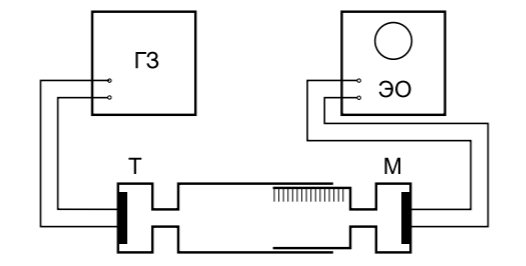
\includegraphics[scale=0.52]{Схема1.png}}
    \caption{Установка для измерения скорости звука при помощи раздвижной трубы}
	\end{figure}
	Первая установка (рис. 1) содержит раздвижную трубу с миллиметровой шкалой. Через патрубок (на рисунке не показан) труба может наполняться воздухом или углекислым газом из газгольдера. На этой установке производятся измерения $\gamma$ для воздуха и для углекислого газа $CO_2$.
	
	\begin{figure}[ht]
	\center{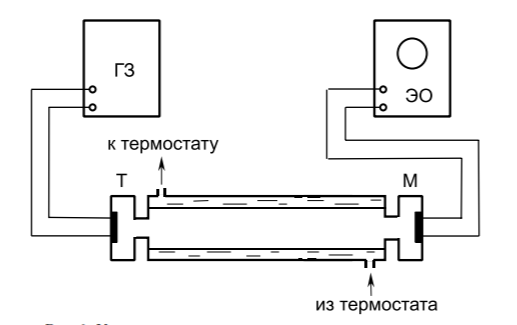
\includegraphics[scale=0.52]{Схема2.png}}
    \caption{Установка для изучения зависимости скорости звука от температуры}
	\end{figure}
	
	Вторая установка (рис. 2) содержит теплоизолированную трубу постоянной длины. Воздух в трубе нагревается водой из термостата. Температура газа принимается равной температуре омывающей трубу воды. На этой установке измеряется зависимость скорости звука от температуры.
	
	\begin{figure}[ht]
	\center{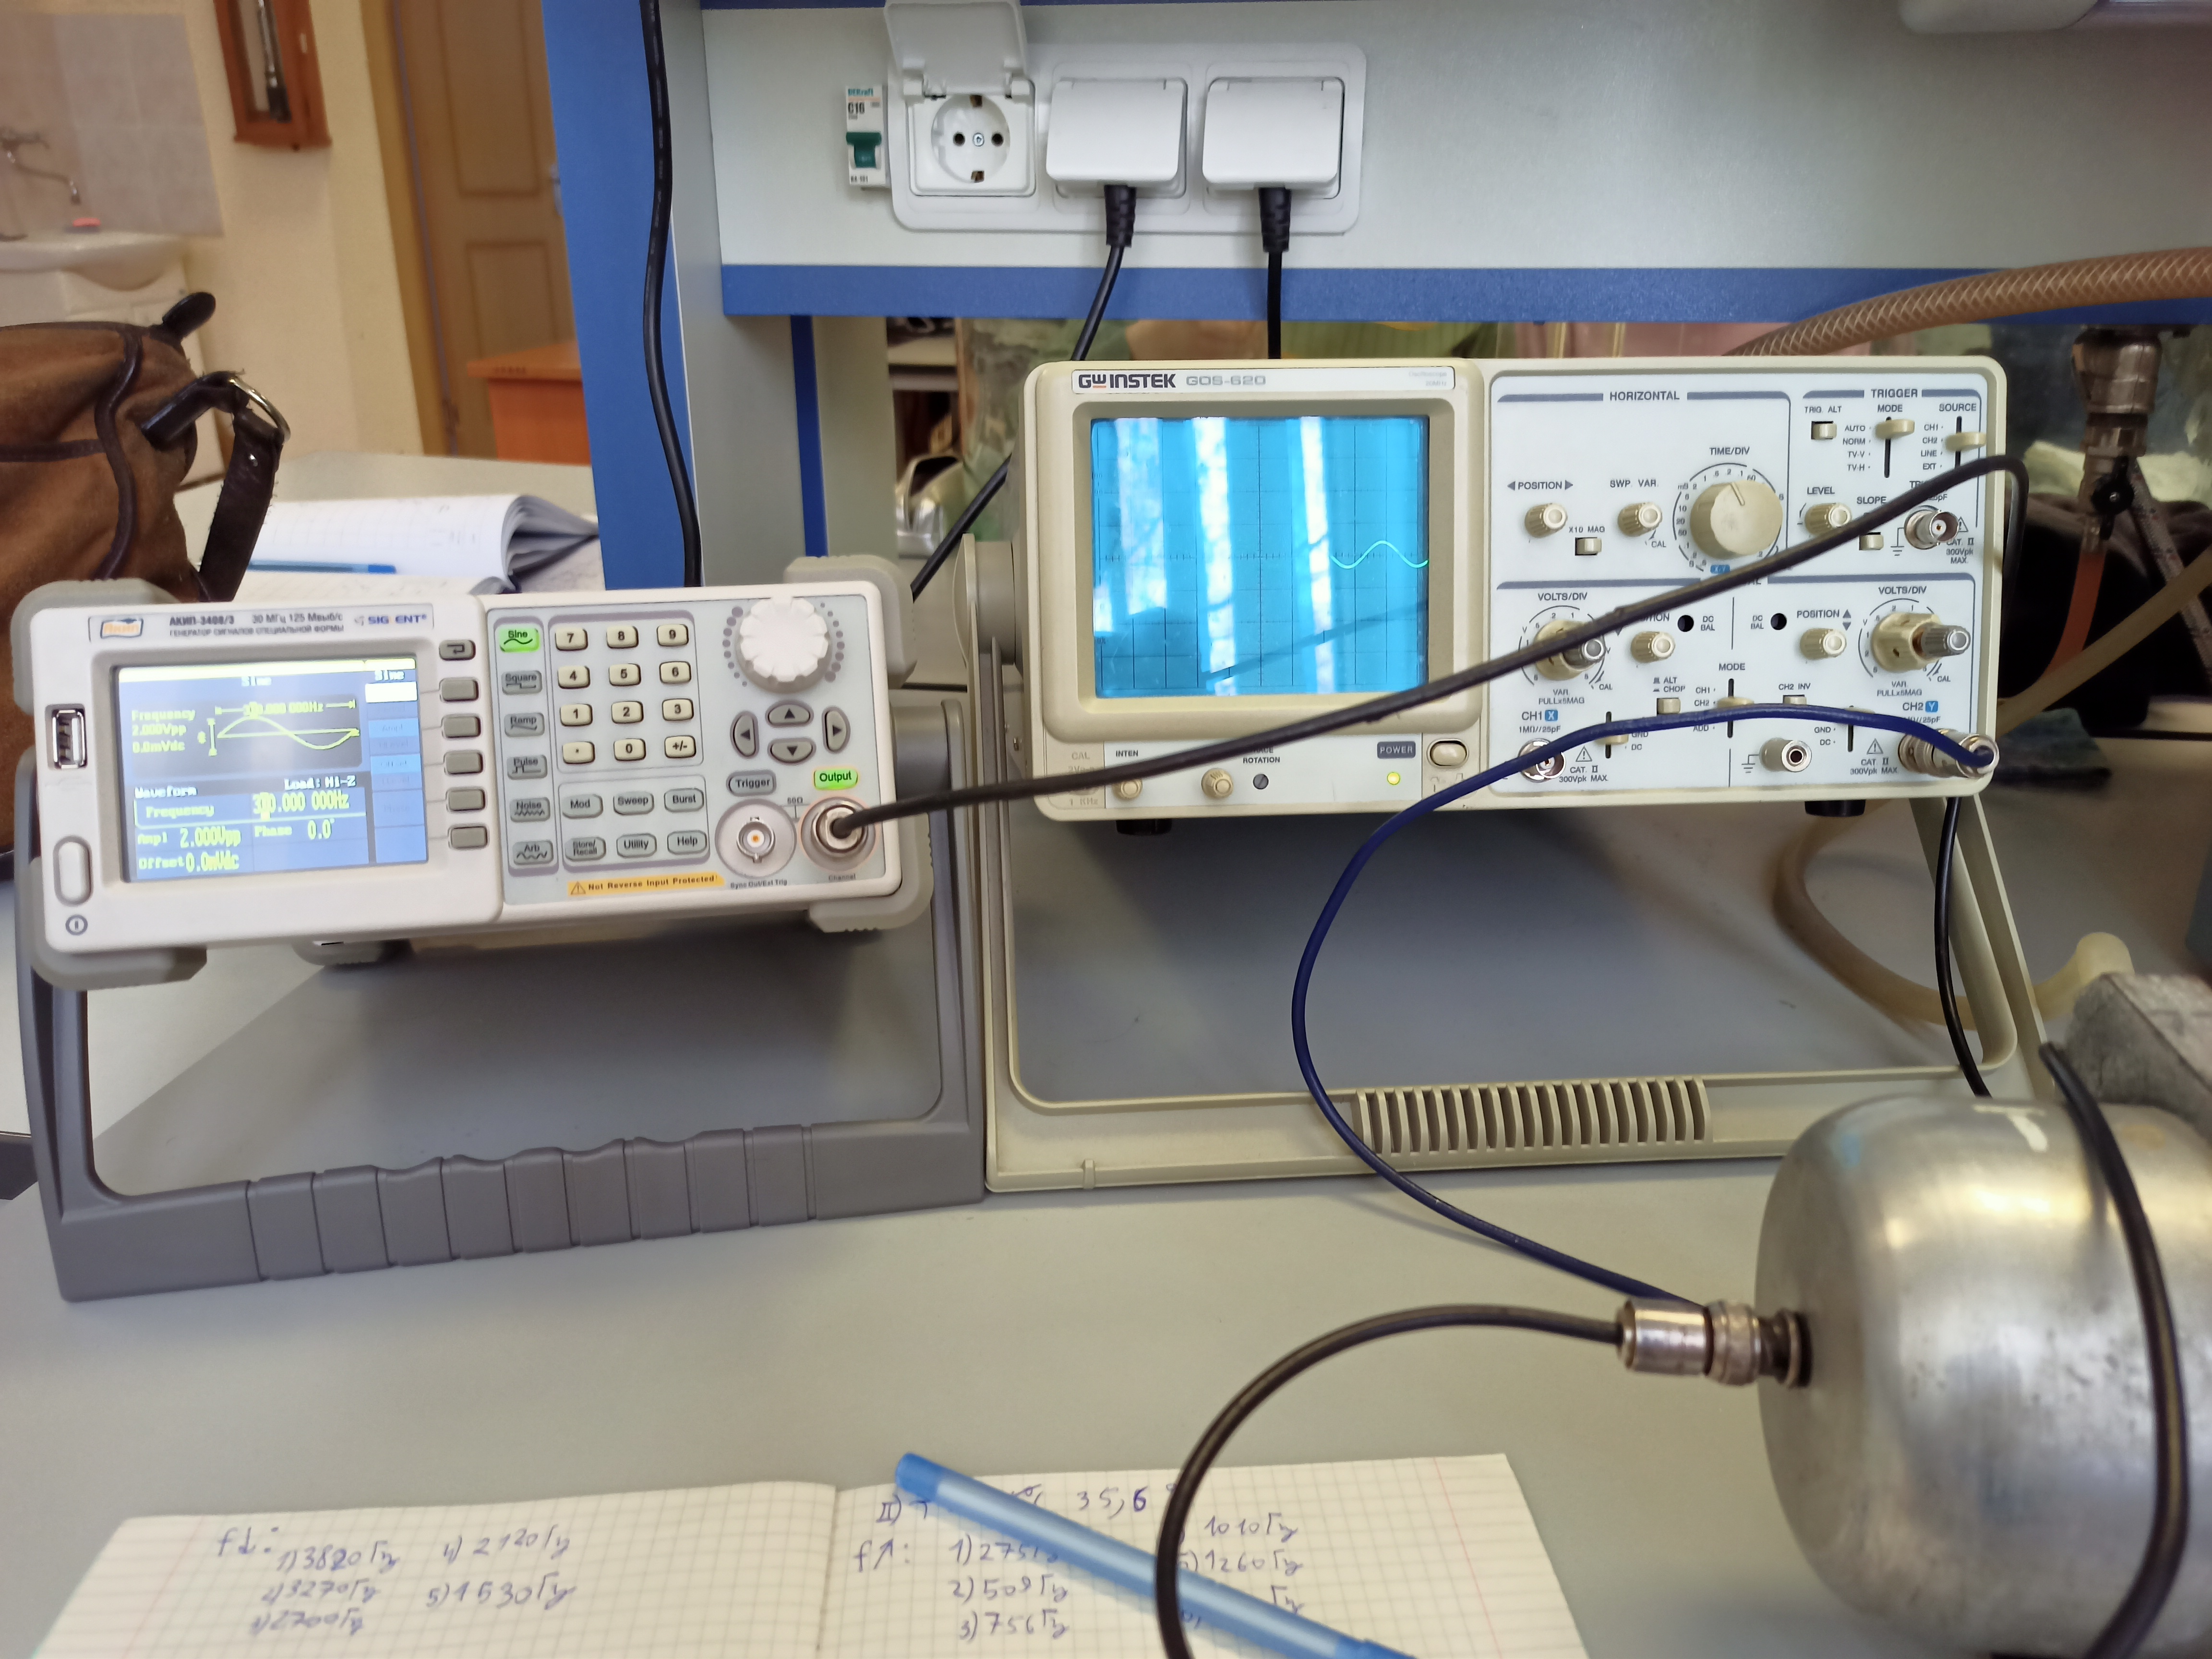
\includegraphics[scale=0.04]{Установка.jpg}}
    \caption{Используемые генератор сигналов и осциллограф (ЭО)}
	\end{figure}



\textbf{Измерения и обработка данных}

		1) Параметры установки:
		$L = 700\pm 5 \; \text{мм}$, t = 24 °C;
		
		Исходя из примерного значения скорости звука ($ \approx 320 \; \frac{\text{м}}{\text{с}}$), рассчитаем, в каком диапазоне частот следует вести измерения, чтобы при удлинении трубы можно было наблюдать x резонансов:
$L = \frac{n\lambda}{2}$, $L + \Delta L = \frac{(n+x)\lambda}{2}$. Поскольку $\Delta L \leq 23 \; {\text{см}}$ - сильнее трубу выдвинуть нельзя, то для 4 резонансов необходимо $\lambda \leq 11.5 \; {\text{см}}$, т.е. $f \geq 2600 \; {\text{Гц}}$ (по ф-ле 2). Для 2 резонансов $\lambda \leq 23 \; {\text{см}}$, т.е. $f \geq 1300 \; {\text{Гц}}$.
		
		2.1) Проведём измерения на первой установке для воздуха.
		Плавно изменяя длину трубы, последовательно зафиксируем все доступные для наблюдения точки резонанса. Измерения проводятся для нескольких частот.
		\begin{table}
		\begin{center}
		\begin{tabular}{|l|l|l|l|l|l|l|l|}
			\hline
			f, Гц & 2518 & 2648 & 2847 & 3123  & 3262
			\\
			\hline
			k &  $\Delta l$, см& $\Delta l$, см& $\Delta l$, см& $\Delta l$, см& $\Delta l$, см
			\\
			
			\hline
			0 & 5,2 & 1,6 & 3,6 & 2,1 & 4,4
			\\
			\hline
			1 & 12,1 & 8,1 & 9,8 & 7,4 & 9,7 
			\\
			\hline
			2 & 19,0 & 14,7 & 16,0 & 13,0 & 15,1
			\\
			\hline
			3 & -- & 21,2 & 22,1 & 18,5 & 20,4
			\\
			\hline
		\end{tabular}
		\caption {Измерения для воздуха}
		\end{center}
		\end{table}
		Значение $\Delta l$ соответствует значению на размеченной подвижной части трубы при измерении как по укорачиванию длины, так и по удлинению.
		Занесём полученные результаты в таблицу 1.
		
		3.1) Изобразим полученные результаты на графиках (см. рис. 4), откладывая по оси абсцисс номер $k$ последовательного резонанса, а по оси ординат — соответствующее удлинение трубы
		$\Delta l$.

		
		На полученных графиках угловой коэффициент прямой определяет длину полуволны. Вычислим с их помощью скорость звука в воздухе, оценим погрешности измерений. Результаты вычислений (по ф-ле 2) см. в таблице 2:
		
			
	\begin{figure}[ht!]
	\center{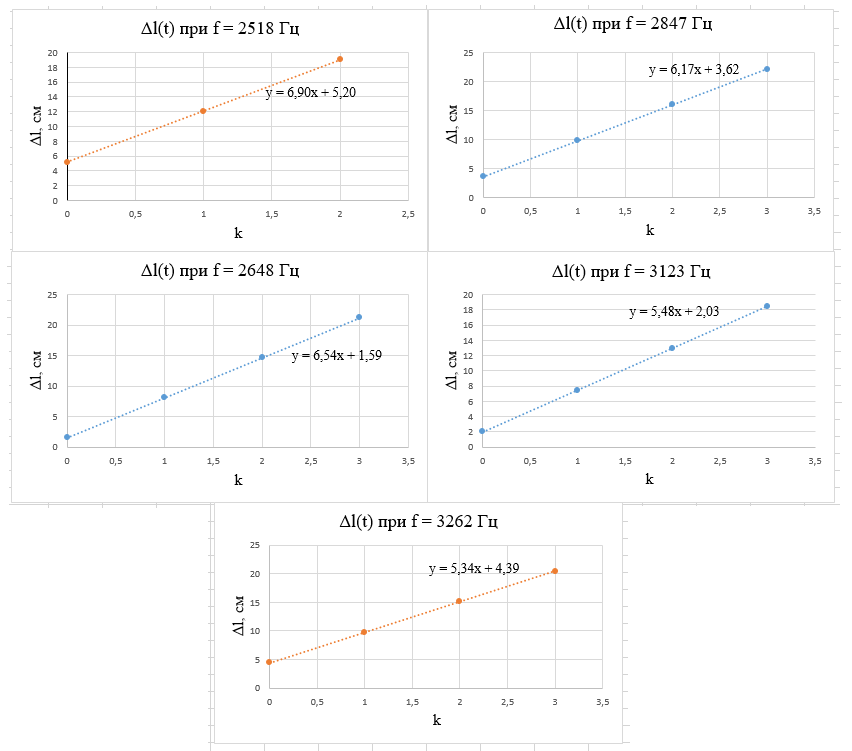
\includegraphics[scale=0.65]{Графики.png}}
    \caption{Зависимость $\Delta l$(k) при различных f для воздуха при 24 °С}
	\end{figure}
		
		\begin{table}
		\begin{center}
		\begin{tabular}{|l|l|l|l|l|l|}
			\hline
			f, Гц & 2518 & 2648& 2847 & 3123 & 3262
			\\
			
			\hline
			$\frac{\lambda}{2},{\text{см}}$ & 6,9 & 6,54 & 6,17 & 5,48 & 5,34
			\\
			\hline
			$c,\frac{\text{м}}{\text{с}}$ & 347,48 & 346,36 & 351,32 & 342,28 & 348,38
			\\
			\hline
			$\sigma_{\lambda}, {\text{см}} $ & 0,05 & 0,05 & 0,05 & 0,05 & 0,05
			\\
			\hline
			$\sigma_{f},{\text{Гц}}$ & 5 & 5 & 5 & 5 & 5
			\\
			\hline
		\end{tabular}
		\caption{результаты обработки для воздуха}
		\end{center}
		\end{table}
		\newpage
		Полученные значения скоростей звука при различных частотах близки.
		Усреднив полученные значения найдём окончательное значение скорости звука в воздухе. Погрешность: $$\sigma_{c} = \sqrt{(\sigma_{\text{случ}})^2+(\sigma_{\text{сист}})^2} = 7,58\frac{\text{м}}{\text{с}}.$$
		Итого, $$c = 347,16 \pm 7,58 \; \frac{\text{м}}{\text{с}}.$$
		Теоретическое значение скорости звука в воздухе при температуре $t = 24 ^\circ C$ равно $$c_{\text{т}} = 345,549 \: \frac{\text{м}}{\text{с}}.$$
		В пределах погрешности эксперементальное значение совпадает с теоретическим.
		
		Из формулы (1) получим: $\gamma=\frac{\mu}{RT} c^2 = 1,42 \pm 0,03,$ что сходится с теоретическим значением $\gamma = \frac{7}{5}$.
		
		2.2) Аналогично пункту 2.1 проведём измерения на первой установке для углекислого газа. Занесём полученные результаты в таблицу 3.
		
		\begin{table}[ht!]
		\begin{center}
		\begin{tabular}{|l|l|l|l|l|l|l|l|l|}
			\hline
			f, Гц & 2326 & 2597 & 2779 & 2938  & 3314 & 3571
			\\
			\hline
			k &  $\Delta l$, см & $\Delta l$, см & $\Delta l$, см & $\Delta l$, см & $\Delta l$, см & $\Delta l$, см
			\\
			
			\hline
			0 & 0,1 & 3,0 & 3,1 & 3,7 & 3,5 & 1,9
			\\
			\hline
			1 & 5,9 & 8,3 & 8,0 & 8,4 & 7,7 & 5,4
			\\
			\hline
			2 & 11,8 & 13,7 & 13,1 & 13,2 & 12,0 & 9,7
			\\
			\hline
			3 & 18,3 & 19,1 & 18,1 & 18,3 & 16,5 & 13,6
			\\
			\hline
			4 & -- & -- & -- & -- & 20,2 & 17,7
			\\
			\hline
			5 & -- & -- & -- & -- & -- & 22,4
			\\
			\hline
		\end{tabular}
		\caption {Измерения для углекислого газа}
		\end{center}
		\end{table}
		
		3.2) Изобразим полученные результаты на графиках (см. рис. 5), откладывая по оси абсцисс номер $k$ последовательного резонанса, а по оси ординат — соответствующее удлинение трубы
		$\Delta l$.

		
		На полученных графиках угловой коэффициент прямой определяет длину полуволны. Вычислим с их помощью скорость звука в воздухе, оценим погрешности измерений. Результаты вычислений (по ф-ле 2) см. в таблице 4:
		
			
	\begin{figure}[ht!]
	\center{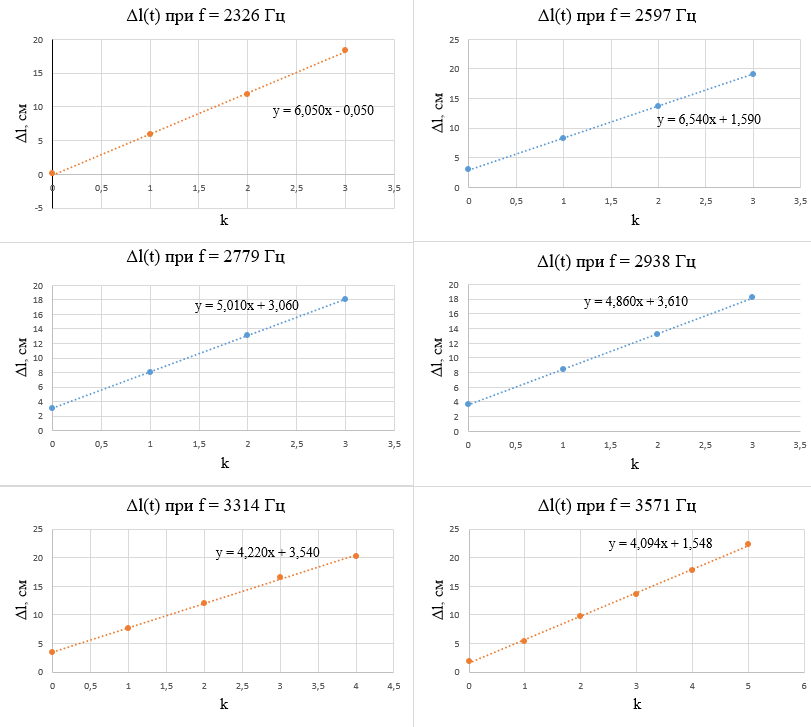
\includegraphics[scale=0.65]{CO2.png}}
    \caption{Зависимость $\Delta l$(k) при различных f для углекислого газа при 24 °С}
	\end{figure}
		
		\begin{table}[ht!]
		\begin{center}
		\begin{tabular}{|l|l|l|l|l|l|l|}
			\hline
			f, Гц & 2326 & 2597 & 2779 & 2938 & 3314 & 3571
			\\
			
			\hline
			$\frac{\lambda}{2},{\text{см}}$ & 6,05 & 6,54 & 5,01 & 4,86 & 4,22 & 4,09
			\\
			\hline
			$c,\frac{\text{м}}{\text{с}}$ & 281,45 & 309,69 & 278,46 & 285,57 & 279,70 & 292,11
			\\
			\hline
			$\sigma_{\lambda}, {\text{см}} $ & 0,05 & 0,05 & 0,05 & 0,05 & 0,05 & 0,05
			\\
			\hline
			$\sigma_{f},{\text{Гц}}$ & 5 & 5 & 5 & 5 & 5 & 5
			\\
			\hline
		\end{tabular}
		\caption{результаты обработки для CO2}
		\end{center}
		\end{table}
		\newpage
		Полученные значения скоростей звука при различных частотах близки.
		Усреднив полученные значения найдём окончательное значение скорости звука в углекислом газе. Погрешность: $$\sigma_{c} = \sqrt{(\sigma_{\text{случ}})^2+(\sigma_{\text{сист}})^2} = 26,98\frac{\text{м}}{\text{с}}.$$
		Итого, $$c = 287,83 \pm 26,98 \; \frac{\text{м}}{\text{с}}.$$
		Теоретическое значение скорости звука в CO2 при температуре $t = 24 ^\circ C$ равно $$c_{\text{т}} = 281,18 \: \frac{\text{м}}{\text{с}}.$$
		В пределах погрешности эксперементальное значение совпадает с теоретическим.
		
		Из формулы (1) получим: $\gamma=\frac{\mu}{RT} c^2 = 1,48 \pm 0,14,$ что сходится с теоретическим значением $\gamma = \frac{7}{5}$.
		
		
		4) Проведём измерения на второй установке. Результаты измерений представлены в таблице 5.
		   
		    \begin{table}[ht!]
			\begin{center}
			\begin{tabular}{|l|l|l|l|l|l|l|l|l|l|}
			\hline
			t, $^\circ C$ & \multicolumn{2}{|c|}{27,0} & \multicolumn{2}{|c|}{35,6}&  \multicolumn{2}{|c|}{45,4}
			\\
			\hline
			k &  $f_1$, Гц & $f_2$, Гц & $f_1$, Гц & $f_2$, Гц & $f_1$, Гц & $f_2$, Гц
			\\
			\hline
			0 & 500 & 502 & 275 & 276 & 275 & 275 
			\\
			\hline
			1 & 744 & 744 & 509 & 510 & 515 & 516 
			\\
			\hline
			2 & 993 & 994 & 756 & 756 & 768 & 768 
			\\
			\hline
			3 & 1240 & 1245 & 1010 & 1010 & 1025 &  1024
			\\
			\hline
			4 & 1490 & 1490 & 1260 & 1259 & 1279 & 1280 
			\\
			\hline
			5 & 1740 & 1735 & 1510 & 1509 & 1534 & 1533 
			\\
			\hline
		\end{tabular}
		\caption{измерения для второй установки}
		\end{center}
		\end{table}
		
		$f_1$ - соответствует значениям, полученным при увеличении частоты, $f_2$ - при уменьшении. Видно, что при обратном ходе данные воспроизводятся.		


		5) Полученные результаты изобразим на графике (см. рис. 6), откладывая
		по оси абсцисс номер резонанса $k$, а по оси ординат — разность между частотой последующих резонансов и частотой первого резонанса: $\Delta f_k = f_{k+1}-f_1.$ Полученный таким образом угловой
		коэффициент прямой на графике определяет величину k = c/2l.
		
\begin{figure}[ht!]
	\center{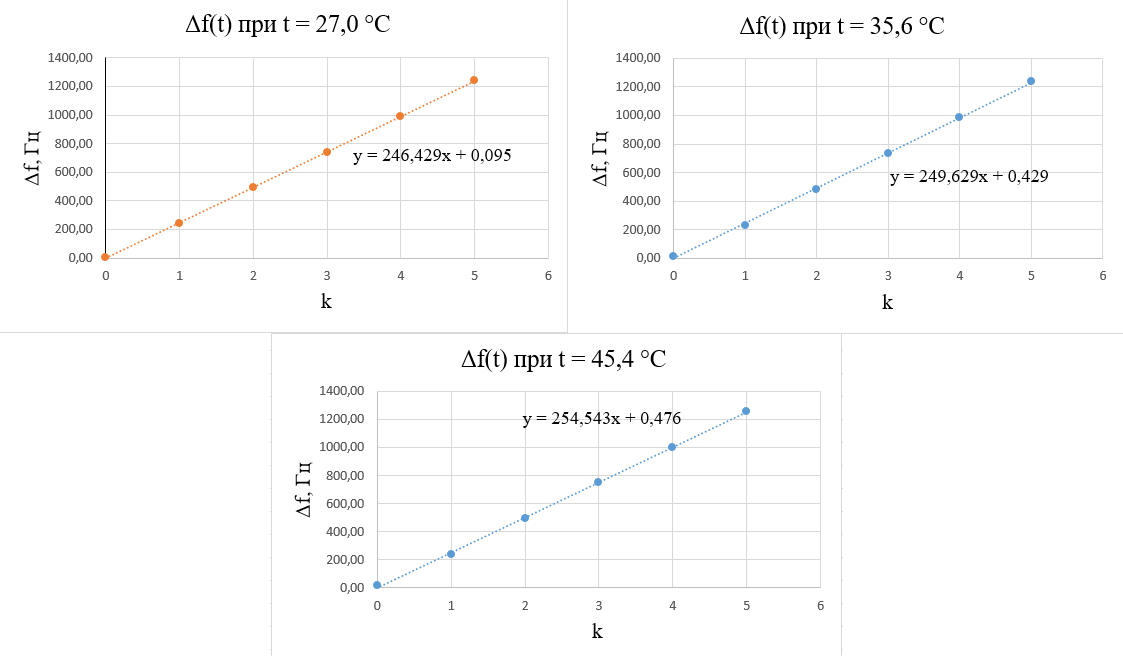
\includegraphics[scale=0.55]{f(t).png}}
    \caption{Зависимость $\Delta f$(k) при различных t для воздуха при l = 700 мм}
	\end{figure}

	Значение $\gamma$ найдём при помощи формулы (1). Результаты вычислений по построенным графикам представлены в таблице 6:
	\begin{table}[ht!]
	\begin{center}
	\begin{tabular}{|l|l|l|l|}
		\hline
		t, $^\circ$ C & 27,0 & 35,6 & 45,4
		\\
		
		\hline
		$k = \frac{c}{2l},{\text{Гц}}$ & 246,43 & 249,63 & 254,54 
		\\
		\hline
		$c,\frac{\text{м}}{\text{с}}$ & 345,00 & 349,48 & 356,36 
		\\
		\hline
		$\sigma_{\text{k}},{\text{Гц}} $ & 9,2 & 7,6 & 8,1 
		\\
		\hline
		$\sigma_{L},{\text{м}} \cdot 10^{-3} $ & 1 & 1 & 1  
		\\
		\hline
		$\sigma_{c},\frac{\text{м}}{\text{с}}$ & 13,44 & 10,24 & 11,34 
		\\
		\hline
		$\gamma$ & 1,38 & 1,38 & 1,39
		\\
		\hline
	\end{tabular}
	\caption{результаты обработки по данным 2 установки (при l = 0,7 м)}
	\end{center}
    \end{table}
    
	Таким образом, $\gamma$ не зависит от температуры и равен $1,38 \pm 0,02$, что в пределах погрешности совпадает  с теоретическим значением $\gamma = 1,40 .$

	
	
\textbf{Выводы:}

	1) В ходе данной работы была найдены длины волн при резонансе звуковых колебаний
в газе, заполняющем трубу (порядка 10 см).

    2) Двумя способами был определён показатель адиабаты $\gamma = \frac{C_p}{C_v}$: при помощи установки с раздвижной трубой (T = const, l меняется) был получен результат $\gamma=\frac{\mu}{RT} c^2 = 1,42 \pm 0,03$; а при помощи установки с термостатом (l = const, T меняется) $\gamma = 1,38 \pm 0,02$. Оба результата сошлись с теоретическим значением $\gamma = 1,40$.
	

	

\end{document}